\chapter{Diskretisierung}

Partielle Differentialgleichungen (PDGn) n-ter Ordnung für skalares $u(x)$ sind von der Form
\begin{equation}
  F(x, t, u(x), Du(x), \dots, D^nu(x))=0, \qquad x\in\Omega\subset\mathbb{R}^d \; .
\end{equation}
Sie unterliegen Randbedingungen (für die Zeitvariable auch Anfangsbedingung genannt), die je nach Problemstellung auf Teilen des Randes formuliert sind. Beispielsweise ist die Auslenkung einer eingespannten Membran am Ortsrand fest, während in der Zeit lediglich für $t_0$ ein Randwert vorliegt (am linksseitigen Rand der Zeitdomäne).

Die LvNG \eqref{eq:lvn} ist eine lineare PDG zweiter Ordnung in $d=2$ Dimensionen. Sie ist weder elliptisch, noch parabloisch, noch hyperbolisch\footnote{Dies ist ersichtlich anhand der Eigenwerte der Koeffizientenmatrix zweiter Ableitungen $T=\text{diag}(0,1,-1)$ für Gleichung \eqref{eq:lvn_first}}.
Ferner bildet $u\in C^2(\Omega)$ in den Raum der komplexen Zahlen ab. Damit unterscheidet sich das Problem bereits grundlegend von den zumeist in der Literatur vorkommenden Problemstellungen. In diesem Kapitel soll ein Verfahren entwickelt werden, welches bislang noch nicht zur Anwendung gekommen ist im Kontext der LvNG: das \emph{Discontinuous-Galerkin}\index{Discontinuous-Galerkin Verfahren} (DG) Verfahren. Die Ausführungen orientieren sich an dem praxisnahen Buch von Hesthaven und Warburton \cite{buch}.

Zunächst wird eine Übersicht über gängige Verfahren zur Lösung von PDGn gegeben. Das DG-Verfahren wird motiviert anhand der jeweiligen Vor- und Nachteile.

\section{Übersicht}
Bei der Diskretisierung einer PDG sind zwei grundlegende Fragestellungen zu berücksichten:
\begin{enumerate}
  \item Auf welche Weise wird die Lösung $u(x,t)$ durch eine diskrete Lösung $u_h(x,t)$ genähert?
  \item Wie ist die Verbindung zwischen diskretisierter Lösung und zugrundeliegender PDG?
\end{enumerate}
Als Folge einer unterschiedliche Beantwortung dieser Fragen wurden zahlreiche Verfahren entwickelt, die jeweils spezifische Vor- und Nachteile aufweisen. Im Folgenden werden in knapper Form drei Verfahren vorgestellt und  gegeneinander verglichen. In dieser Reihenfolge nimmt die Komplexität zu, denn die Schwächen des einen Verfahrens führen jeweils zu der nächst allgemeineren Formulierung.

\subsection{Finite Differenzen}\index{Finite Differenzen}\label{sec:FD}
Die partiellen Ableitungen werden bei diesem Verfahren durch eine endliche (finite) Anzahl von Differenzen genähert. Zur Formulierung der n-ten Ableitung einer Funktion $f(x)$ im Punkt $x_0$ wird die zugehörige Taylorreihe bis zur n-ten Ordnung verwendet. Der Punkt $x_0$ entstammt einem Gitter, welches das Gebiet $\Omega$ diskretisiert. Dieser Ansatz setzt inhärent voraus, dass eine Funktion sich hinreichend genau durch ein lokales Polynom niedriger Ordnung nähern lässt. Damit ist zeitgleich Frage (1) beantwortet.

Die Antwort auf die zweite Frage bestimmt dann die Koeffizienten der lokalen Polynome. Durch Einsetzen der Näherung $u_h(x,t)$ in die PDG folgt ein Residuum
\begin{equation}
  \mathcal{R}(x,t)\equiv F(x,t, u_h(x), Du_h(x), \dots, D^nu_h(x,t)) \; ,
\end{equation}
welches i.A. nicht verschwindet, denn sonst wäre ${u_h(x,t) = u(x,t)}$ die exakte Lösung. Zur Bestimmung der Koeffizienten (Freiheitsgrade) wird daher beispielsweise gefordert, dass auf den Gitterpunkten ${\mathcal{R}(x^k,t)=0}$ verschwindet.

Das Verfahren ist besonders leicht zu implementieren. Es ist robust, effizient und wird von einer umfangreichen Literatur gestützt. Für zeitabhängige Probleme folgt aus der Ortsdiskretisierung eine explizite semidiskrete Form, was eine Flexibilität in der Wahl der Zeitschritt-Methode ermöglicht. In höherdimensionalen Problemen $d>1$ erfordert das Verfahren jedoch eine Tensorprodukt-Struktur der Basisfunktionen, sodass letztlich komplexe Geometrien $\Omega\subset{\mathbb{R}^d}$ nicht gut abgebildet werden können. Ferner führen Unstetigkeiten in den Randbedingungen oder internen Schichten (wie zum Beispiel der Potentialsprung in Abbildung \ref{fig:pot1}) zu Problemen aufgrund der simplen, zugrundeliegenden Diskretisierung.

\subsection{Finite Volumen}\index{Finite Volumen}
Für erhöhte geometrische Flexibilität und insbesondere für nichtlineare Erhaltungsgleichungen eignet sich das Finitive Volumen (FV) Verfahren. Das Gebiet $\Omega$ wird dabei in Zellen aufgteilt, zumeist Simplizes. Die approximative Lösung $u_h(x,t)$ wird als Konstante $\bar{u}^k(t)$ innerhalb einer Zelle $k$ gesetzt. Die PDG wird lokal über jede Zelle integriert, wobei auftretende Divergenzterme mit Hilfe des Gaußschen Satzes in Oberflächenterme überführt werden. Für diese Terme müssen geeignete Flüsse gefunden werden und diese Wahl führt zu unterschiedlichen Verfahren. Da der Fluss in eine Zelle hinein demjenigen aus der Nachbarzelle heraus entspricht, sind die FV Verfahren konservativ.

Während wegen der Flexibilität bezüglich Geometrie und Wahl des Flusses die FV Verfahren sehr erfolgreich sind, offenbart die Forderung nach Verbesserung der Genauigkeit ein fundamentales Problem: im mehrdimensionalen müsste die geometrische Flexibilität wieder fallengelassen werden. Um nämlich $u_h(x,t)$ als Polynom vom Grad $N$ zu entwickeln und somit ${N+1}$ Koeffizienten zu finden, müssen zellübergreifende Informationen gesammelt werden aus mindestens ${N+1}$ Zellen (der sogenannten \emph{stencil} wird ausgeweitet). Dadurch wird eine spezielle Gitterstruktur erforderlich, weshalb geometrische Flexibilität nicht länger gewährleistet ist.

Im eindimensionalen Fall $d=1$ ist eine Erhöhung der Genauigkeit jedoch möglich und es soll an dieser Stelle betont werden, dass die LvNG ebenso mit einem zweistufigen FV Verfahren und Polynomgraden ${N_x,N_y > 1}$ gelöst werden kann. Die Flexibilität des Gitters ist im Falle eines hybdriden FV/DG-Verfahrens ohnehin nicht gegeben (vgl. Kapitel \todo{Referenz}).

\subsection{Finite Elemente}\index{Finite Elemente}
Der Übergang zu den Finite Elemente Methoden (FEM) geschieht, indem die approximative Lösung innerhalb einer Zelle nicht mehr als konstant gesetzt wird. Erhöhung der Genauigkeit durch Erhöhung der Freiheitsgrade ist dann ohne weiteres möglich, indem ähnlich wie beim FD Verfahren das Residuum auf den inneren Interpolationspunkten einer jeden Zelle orthogonal zu allen Testfunktionen sein soll (vgl. Kapitel \ref{sec:FEM}). Die numerische Lösung $u_h(x,t)$ wird also als lokales Polynom auf jeder Zelle angesetzt, wobei sogar der Polynomgrad von Zelle zu Zelle verschieden sein kann (sogenannte \emph{hp-adaptivity}). Die Wahl der Räume für Basis- und Testfunktionen führt zu unterschiedlichen FEM Verfahren. Werden an die Polynome zellübergreifende Stetigkeitsanforderungen gestellt, so führt dies zu den \emph{Continuous Galerkin} (CG)\index{Continuous Galerkin (CG)} Methoden.

Ein Nachteil ist hier für zeitabhängige Probleme die implizite Form der Massenmatrix, die eine Invertierung in jedem Zeitschritt erfordert. Ferner führen Schocks und Unstetigkeiten, wie sie in hyperbolischen Erhaltungsgleichungen auftreten können, zu Problemen \cite{dolejvsi2015discontinuous}. In FD- bzw. FV-Verfahren werden solche Umstände durch ein \emph{Upwind Scheme}\index{Upwind Scheme} bzw. einen \emph{Upwind Flux}\index{Upwind Flux} berücksichtigt. Indem die oben genannte Stetigkeitsanforderung fallen gelassen wird, lassen sich die Vorteile von FV und CG-FEM kombinieren durch die sogenannten  \emph{Discontinuous Galerkin}\emph{Discontinuous Galerkin (DG)} (DG) Methoden. Genau wie bei den FV Verfahren ist auch für die DG Methoden die Wahl eines geeigneten Flusses das Herzstück.

Die Abbildung \ref{fig:vergleich_hest} zeigt schematisch die Vor- und Nachteile der genannten Verfahren. Zahlreiche Entwicklungen und Erweiterungen überwinden die Nachteile häufig und es gibt daneben eine Reihe weiterer Eigenschaften, die zumeist problemabhängig sind und daher in dieser Übersicht nicht erwähnt werden können.
\todo{Scan}


\section{DG-Verfahren für die LvNG}
Für zeitabhängige PDGn mit Dimensionalität $d>1$ gibt es prinzipiell zwei verschiedene Möglichkeiten der Diskretisierung.
\begin{itemize}
  \item Die jeweiligen Orts-Koordinaten werden sukzessive behandelt -- dieses Vorgehen wird als \emph{Methode der Geraden}\index{Methode der Geraden} bezeichnet. Dabei können die einzelnen Richtungen auch mit unterschiedlichen Methoden diskretisiert werden, was im Folgenden als \emph{Hybridverfahren}\index{Hybridverfahren} bezeichnet werden soll. Das resultierende Gitter ist stets ein Rechteckgitter, was wie bereits in Kapitel \ref{sec:FD} erwähnt geometrische Flexibilität nicht zulässt. Andererseits ist dies für rechteckige Gebiete $\Omega$ unkritisch.
  \item Die Orts-Koordinaten werden mit einem einzigen Verfahren diskretisiert -- die Basisfunktionen ergeben sich dann nicht mehr aus einem Tensorprodukt, sondern sind direkt $d$-dimensional.
\end{itemize}
Die Abbildung \ref{fig:methodeDerGeraden} veranschaulicht das Vorgehen.
\begin{figure}
  \centering
  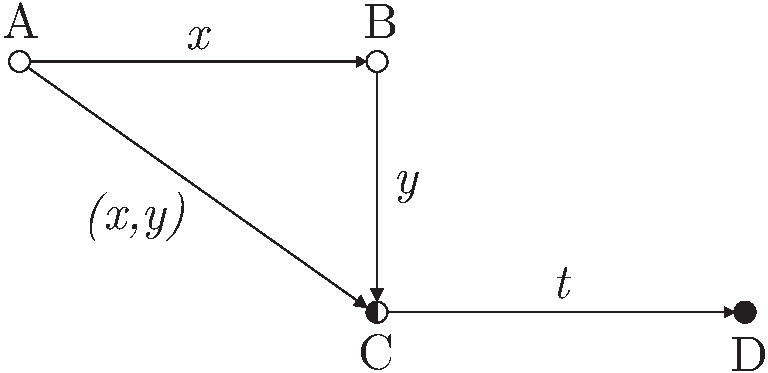
\includegraphics[width=0.7\textwidth]{files/methodeDerGeraden.pdf}
  \caption{Zwei verschiedene Möglichkeiten, zur semidiskreten Form C zu gelangen. Der Weg über B entspricht dabei der \emph{Methode der Geraden}. Im Punkt C verbleibt ein System gewöhnlicher DGLn, welches mit einem geeigneten Zeitschrittverfahren gelöst wird.}
  \label{fig:methodeDerGeraden}
\end{figure}

\subsection{DG/FV Hybridverfahren}
In natürlichen Einheiten kann die bezüglich $y$ diskretisierte LvNG allgemein durch
\begin{equation}
  {A}^y u_t(x,t) + {B}^y u_x(x,t) + {C}^y(x)u(x,t) = 0
  \label{eq:qschema}
\end{equation}
geschrieben werden. Die Matrizen  ${A}^y$, ${B}^y$ und ${C}^y$ resultieren in diesem Abschnitt aus einem FV Verfahren, können aber ebenso anderen Verfahren entstammen.

Dem FV Ansatz in \cite{lukas1} folgend wird das Intervall ${[-L_y/2,+L_y/2]}$ in $K_y$ Zellen unterteilt. Hieraus ergeben sich demnach $K+1$ \emph{interfaces} ${y_{\nicefrac{1}{2}}, y_{\nicefrac{3}{2}}, \dots, y_{K_y + \nicefrac{1}{2}} = -L_y/2, -L_y/2+\Delta y_1,\dots,+L_y/2}$.
Hierbei ist $\Delta y_i$ das Volumen der i-ten Zelle. Der Ansatz führt zu simplen Matrizen der Dimension ${K_y\times K_y}$ mit nicht verschwindenden Einträgen gemäß
\begin{equation}
  \begin{aligned}
  {A}^y_{i,i} &= \Delta y_i \\
  {B}^y_{i,i+1} &= -\frac{i}{2} \qquad
  {B}^y_{i+1, i} = +\frac{i}{2}  \\
  {C}^y_{i,i}(x) &= \mathrm{i} \frac{\Delta y_i}{4} (B(x, y_{i+\nicefrac{1}{2}}) + B(x, y_{i-\nicefrac{1}{2}}))  \\
  {C}^y_{i,i+1}(x) &= C^y_{i+1,i}(x) = \mathrm{i} \frac{\Delta y_i}{4} B(x, y_{i+\nicefrac{1}{2}})  \; .
  \end{aligned}
\end{equation}
Dieses Schema impliziert, dass $u(x,t)$ an den \emph{interfaces} als Mittelwert von rechts- und linksseitiger Zelle angenommen wird. Des weiteren sind  homogene Dirichlet Randbedingungen angenommen, also ${u(x,y_{\nicefrac{1}{2}}, t) = u(x,y_{K_y+\nicefrac{1}{2}}, t) = 0}$.

Die Matrix $B^y$ kann analytisch diagonalisiert werden. Es ist ${B^y = R\Lambda^y R^{\dagger}}$ mit der Diagonalmatrix
\begin{equation}
  \Lambda^y_{m,n} = \cos\left(\frac{2\pi n}{K_y+1}\right)\delta_{m,n}   \qquad m,n = 1,\dots,K_y
\end{equation}
und zugehörigen Eigenvektoren
\begin{equation}
  R_{m,n} = i^m \sin\left(\frac{mn\pi}{K_y +1} \right)   \qquad m,n = 1,\dots,K_y \; .
\end{equation}





% Die in Abbildung \ref{fig:pot1} eingezeichneten Längen werden wie in \cite{lukas1} zu
% \begin{align}
%   L_1 &= \SI{6}{\nano\meter}\\
%   L_2 &= \SI{5}{\nano\meter}\\
%   L_U &= \SI{30}{\nano\meter} \; .
% \end{align}
% gewählt. Hierin ist $L_U$ die Länge, über der die Spannung $U$ abfällt.

\todo{Idee: TF-Lösung für Überlagerung von l und r zeigen.}

% \section{Mathematische Aspekte der \lvn}
% Die eindimensionale Wellenfunktion $\Psi(x)$ eines Teilchens ist ein Vektor des unendlich-dimensionalen Hilbertraums $L^2(\mathbb{R})$ mit dem üblichen Skalarprodukt
% \begin{align}
%   \bra{\Psi}\ket{\Phi} = \int_{\mathbb{R}} \Psi^*(x)\Phi(x) \diff x \; .
% \end{align}
% Beschränken wir uns auf ein Rechengebiet $L$, so ist entsprechend $\Psi(x) \,\in\,L^2(L)$. Diskretisieren wir ferner das System, so wird der Hilbertraum endlichdimensional mit Dimension $N$. Dann ist die Dichtematrix in Gleichung \eqref{eq:lvn} eine Matrix der Form $\mathbb{C}^N \times \mathbb{C}^N$ und der Liouville-Operator ein "Superoperator" \cite{frensley2} der Form $(\mathbb{C}^N \times \mathbb{C}^N)\times(\mathbb{C}^N \times \mathbb{C}^N)$.
% Letztlich wird numerisch gesehen $N^2$ der Anzahl Freiheitsgrade entsprechen und die \lvn wird wieder eine Matrix-Vektor-Gleichung sein. Dazu wird $u(x,y)$ nicht als Matrix, sondern als Vektor der Länge $N^2$ geschrieben.
% \todo{Eigenschaften von B(x,y) und A. Hermitizität von $\mathcal{L}$ (frensley).}


% Idee: Bild zu Methode der Geraden vs. 2d approach    x,y,t--------- x,t
%                                                           \         |
%                                                                \    |
%                                                                     t  ---------  num. Lsg
